
\chapter{Experimental Results}
\label{chap:validation}
This chapter presents the evaluation of the key subsystems developed for the GolfBot project. The performance of each component was assessed through a series of quantitative and qualitative tests designed to validate its effectiveness in fulfilling its designated role.

\section{Computer Vision System Evaluation}
\label{sec:cv_evaluation}
The performance of the computer vision system was evaluated in two stages. First, a quantitative analysis of the trained YOLOv11-seg model was conducted using the hold-out test dataset to assess its detection accuracy. Second, a qualitative real-world test was performed to observe the model's robustness in a live operational scenario.

\subsection{Divot Detection Accuracy}
\label{ssec:cv_accuracy}
The accuracy of the trained YOLOv11-seg model was evaluated using standard metrics in the field of object detection. The primary metrics used are Precision (the accuracy of the positive predictions) and Recall (the ability of the model to find all relevant instances).

The relationship between these two metrics is best captured by the Precision-Recall (P-R) curve, shown in Figure \ref{fig:pr_curve}. A model that is close to the top-right corner of the graph maintains high precision even as it finds a high percentage of the true objects (high recall). The area under this curve is summarized by the Mean Average Precision (mAP) score, which is the single most important metric for evaluating object detector performance. As shown in the figure, the model achieved an impressive **mAP@0.5 score of 0.954** across all classes, indicating a high level of accuracy on the test dataset.

\begin{figure}[h!]
    \centering
    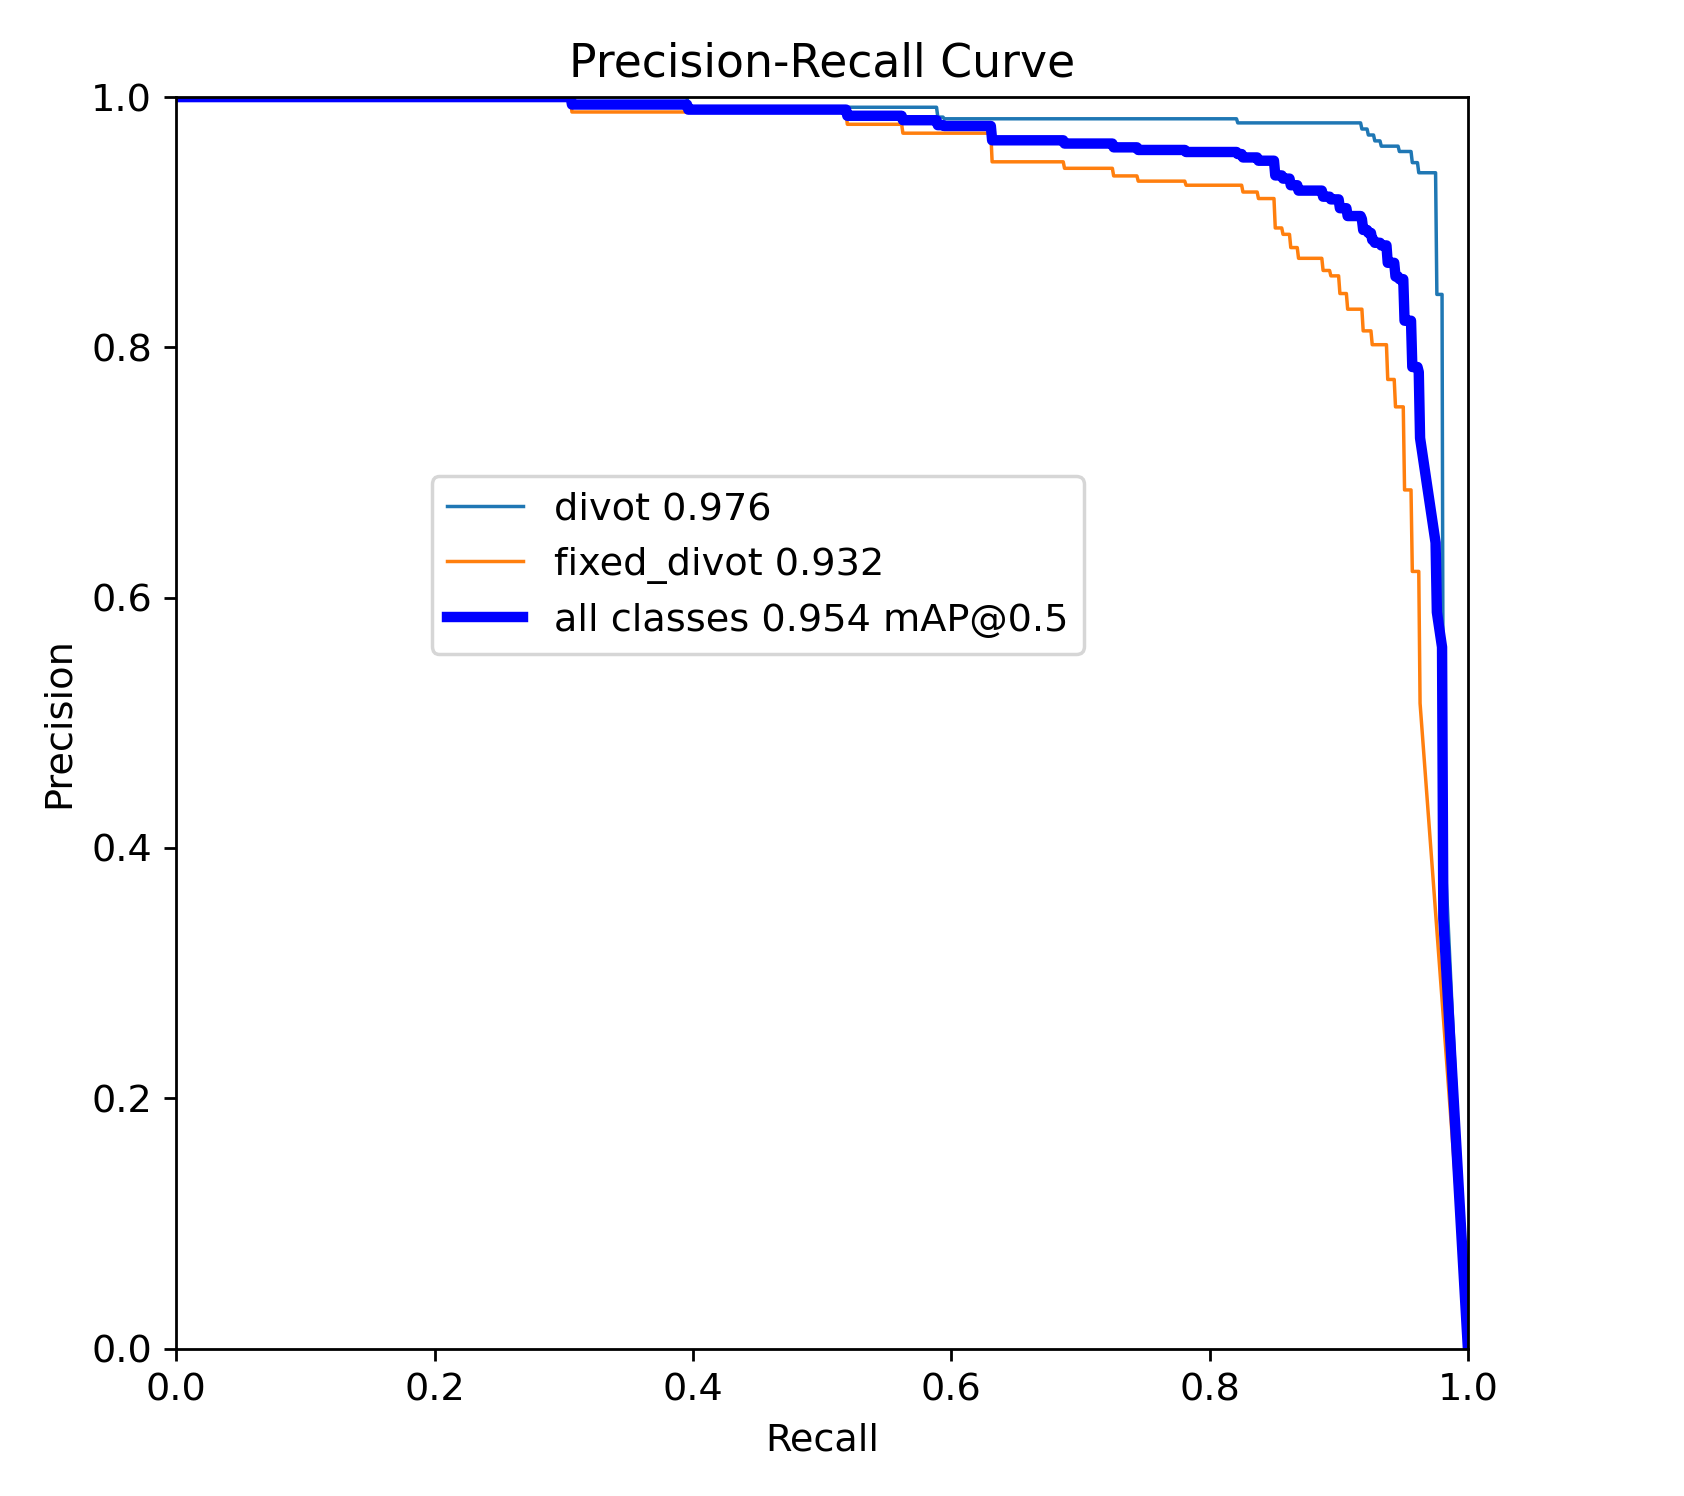
\includegraphics[width=0.8\linewidth]{figures/precision_recall_curve.png}
    \caption{The Precision-Recall (P-R) curve for the trained YOLOv11-seg model. The overall mAP@0.5 of 0.954 demonstrates the model's high accuracy.}
    \label{fig:pr_curve}
\end{figure}

To better understand the model's classification performance, a confusion matrix was generated, as shown in Figure \ref{fig:confusion_matrix}. This matrix shows what categories the model predicted versus the true categories. The normalized version shows that the model is highly effective at its primary task:
\begin{itemize}
    \item It correctly identified true \texttt{divot} instances 98\% of the time.
    \item It correctly identified true \texttt{fixed\_divot} instances 90\% of the time.
    \item The most common error was misclassifying a \texttt{fixed\_divot} as background (10\% of the time), which is an acceptable failure mode as it avoids attempting to repair an already fixed divot.
\end{itemize}

\begin{figure}[h!]
    \centering
    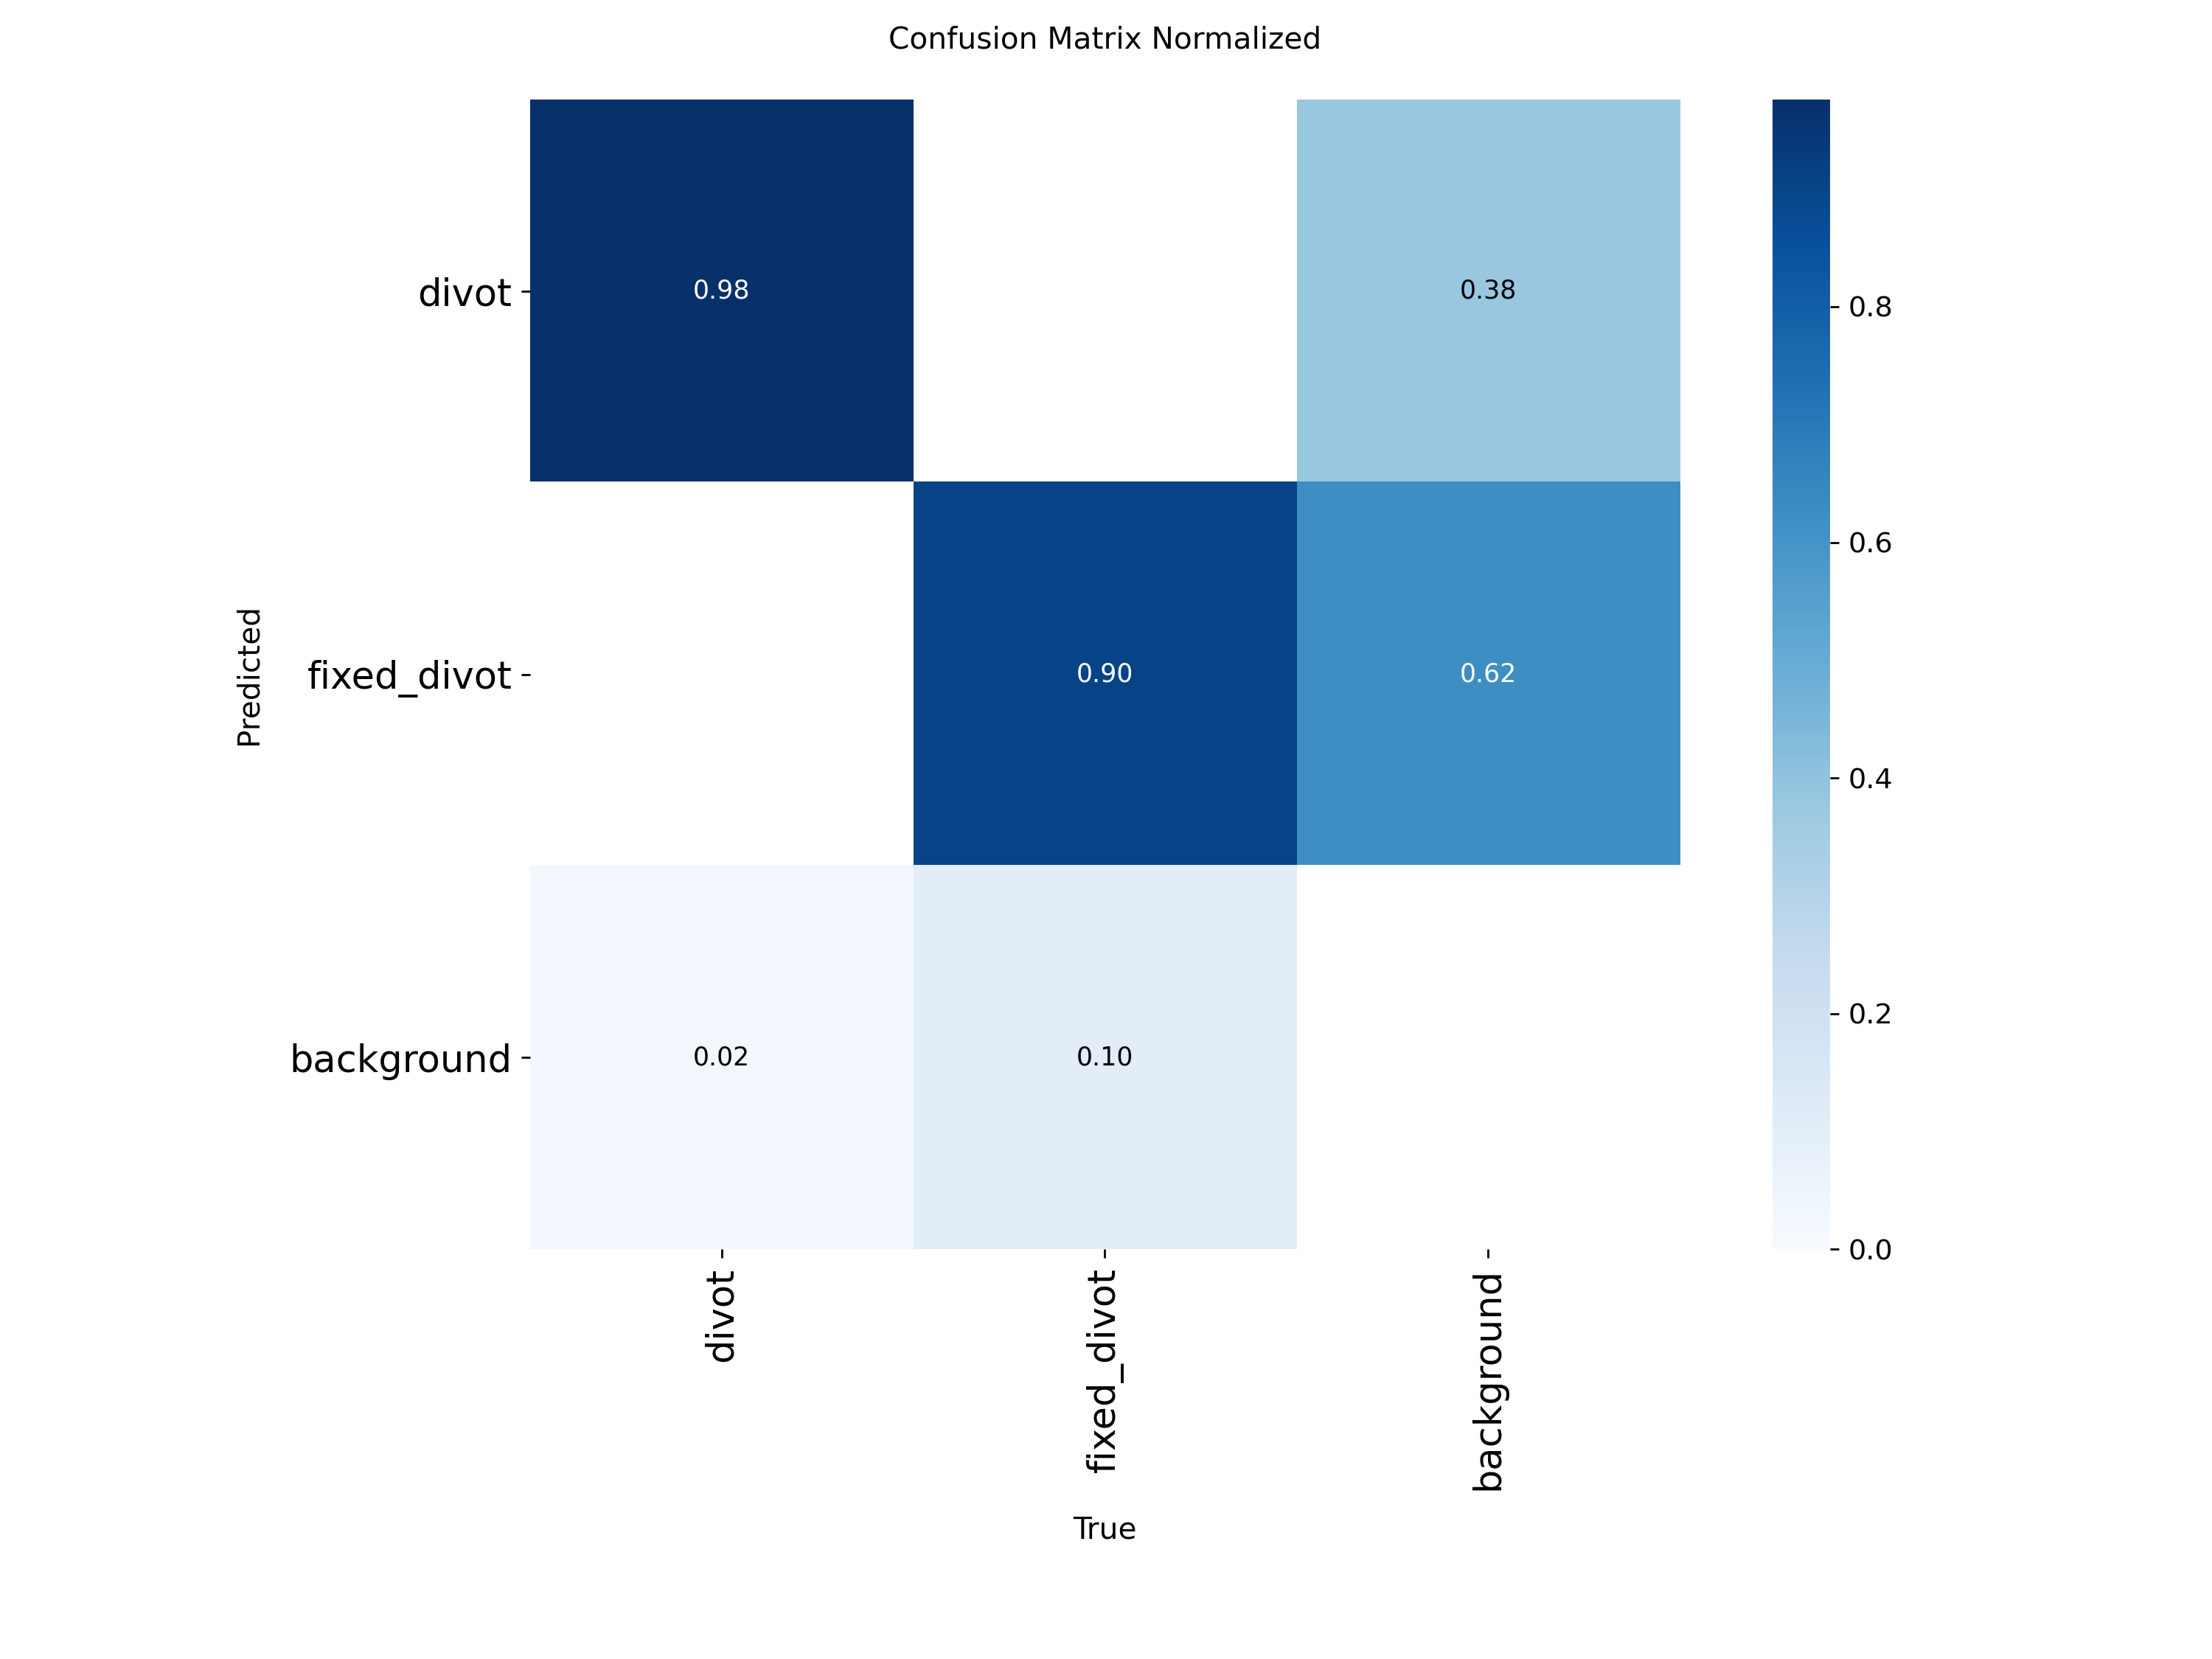
\includegraphics[width=0.7\linewidth]{figures/confusion_matrix_normalized.png}
    \caption{Normalized confusion matrix showing the model's classification accuracy on the test set.}
    \label{fig:confusion_matrix}
\end{figure}

In addition to these quantitative metrics, a qualitative comparison of the model's performance on the unseen validation set is provided in Figure \ref{fig:validation_comparison}. The figure directly compares the ground truth labels (a) with the model's predictions (b) on the same set of images. The high degree of visual similarity between the two provides strong qualitative evidence of the model's effectiveness. The model successfully identifies a variety of divot shapes and sizes under different lighting conditions.

\begin{figure}[h!]
    \centering
    \begin{subfigure}[b]{0.49\textwidth}
        \centering
        \includegraphics[width=\textwidth]{figures/val_batch1_labels.png}
        \caption{Ground truth labels}
        \label{fig:val_labels}
    \end{subfigure}
    \hfill % This creates a small, flexible space between the images
    \begin{subfigure}[b]{0.49\textwidth}
        \centering
        \includegraphics[width=\textwidth]{figures/val_batch1_pred.png}
        \caption{Model's predictions}
        \label{fig:val_preds}
    \end{subfigure}
    \caption{Visual comparison of ground truth labels (a) and the model's predictions (b) on a sample batch of images from the unseen validation set.}
    \label{fig:validation_comparison}
\end{figure}

These quantitative and qualitative results confirm that the model is well-trained and highly capable of distinguishing between divots, fixed divots, and the background environment. Additional performance graphs, including the F1-Confidence curve, are provided in Appendix \ref{chap:appendix_a}.
% \subsection{Real-World Performance}
% \label{ssec:cv_real_world}
% While quantitative metrics validate the model's performance on a static dataset, a qualitative test was conducted to assess its performance in a dynamic, real-world scenario. A full on-course test with the integrated robot was not feasible due to the limitations of the Wumpus platform's wheels, which lacked sufficient traction for consistent navigation on turf.

% Instead, a live test of the vision system was performed. The \texttt{/divot\_detector} ROS 2 node was run on the robot, and the camera was manually pointed at various test subjects in a garden setting that simulated a golf course fairway. This test was designed to evaluate the model's robustness to novel viewpoints, motion blur, and variations in lighting that were not present in the training data.

% The system performed well, successfully identifying and segmenting both new, unseen divots and sand-filled patches in real-time. The visual output from the GUI, as seen in Figure \ref{fig:real_world_examples}, demonstrates the model's ability to generalize to new data. The primary observation was that detection confidence scores tended to be lower in cases of harsh shadows or when a divot was partially obscured by long grass, which is an expected limitation. Overall, this qualitative test confirmed that the implemented computer vision pipeline is robust and suitable for real-world deployment.

% \begin{figure}[h!]
%     \centering
%     \includegraphics[width=\linewidth]{figures/validation_examples.png}
%     \caption{A collage of real-world detection examples from the validation set, showing the model correctly identifying and segmenting both `divot` (blue mask) and `fixed_divot` (cyan mask) instances under various conditions.}
%     \label{fig:real_world_examples}
% \end{figure}

\section{Depth and Volume Estimation Accuracy}
\label{sec:volume_evaluation}
A key objective of the computer vision system is not just to detect divots, but also to estimate their physical size to determine the required amount of repair material. To validate the accuracy of the depth-based measurement algorithm, a controlled experiment was conducted.

\textbf{Experimental Setup.}
As a real-world divot has an irregular shape and depth, a standardized target was used for this test. A shallow, rectangular box with ground-truth dimensions of 11 cm x 5 cm x 2 cm was placed on a flat surface. The Intel RealSense camera was mounted on a tripod at a fixed height, pointing directly down at the target, as shown in Figure \ref{fig:volume_test_setup}. A custom Python script (\texttt{divot\_depth\_seg\_mask\_est.py}) was developed to perform the measurement. This script uses HSV color thresholding to segment the dark interior of the box (simulating a divot) from the light-colored "ground" plane around it.

\begin{figure}[h!]
    \centering
    \begin{subfigure}[b]{\textwidth}
        \centering
        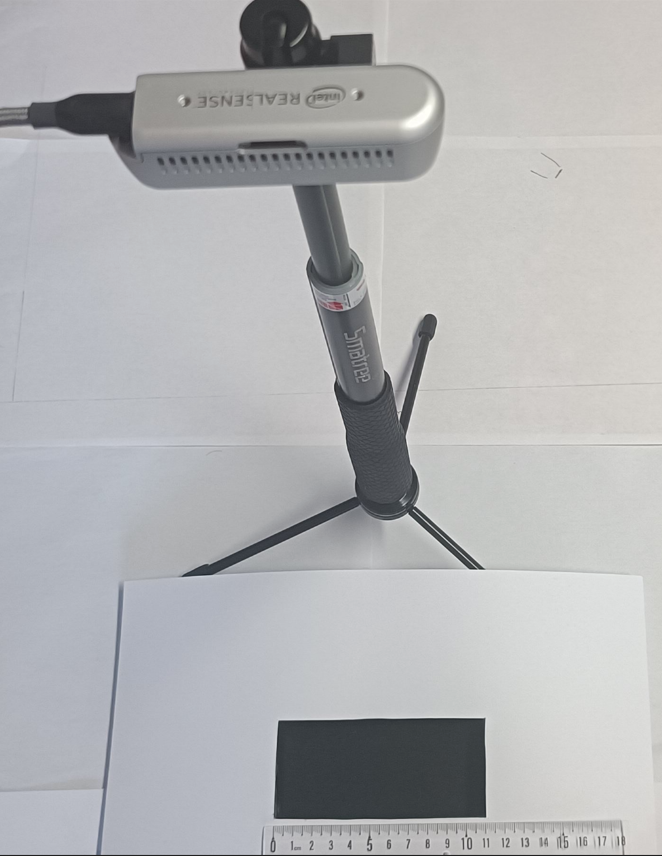
\includegraphics[width=0.6\linewidth]{figures/volume_test_setup.png}
        \caption{Experimental setup showing the camera positioned over a target of known dimensions.}
        \label{fig:volume_test_setup_img}
    \end{subfigure}
    
    \vspace{0.5cm} % Add some vertical space between the setup and the results

    \begin{subfigure}[b]{0.49\textwidth}
        \centering
        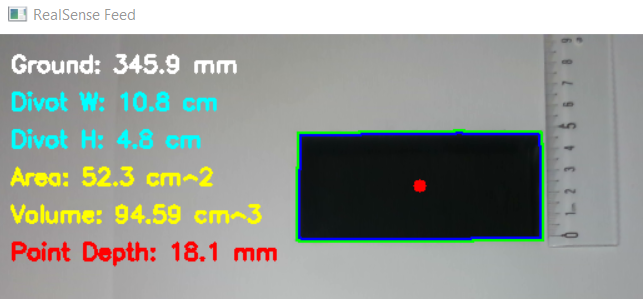
\includegraphics[width=\linewidth]{figures/volume_test_result_5_fix.png}
        \caption{Result from Trial 1.}
        \label{fig:volume_test_result_1}
    \end{subfigure}
    \hfill
    \begin{subfigure}[b]{0.49\textwidth}
        \centering
        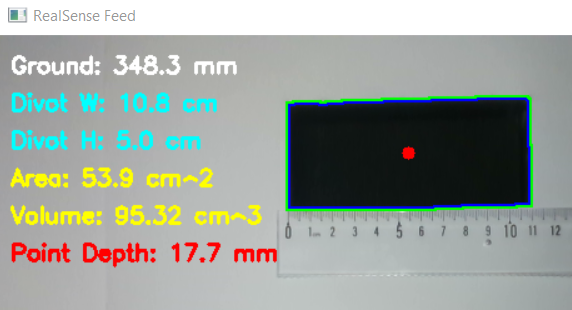
\includegraphics[width=\linewidth]{figures/volume_test_result_11_fix.png}
        \caption{Result from Trial 2.}
        \label{fig:volume_test_result_2}
    \end{subfigure}
    \caption{The controlled experiment to validate the volume estimation algorithm. The setup (a) and two sample results (b, c) showing the system's calculated dimensions and volume.}
    \label{fig:volume_test_setup}
\end{figure}

\textbf{Measurement Algorithm.}
The script calculates the volume using a pixel-by-pixel integration method. It first determines the average depth of the surrounding ground plane. Then, for each pixel inside the segmented divot mask, it calculates the depth difference relative to this ground plane. The real-world area of each pixel is estimated using the camera's intrinsic parameters. The total volume is the sum of the volume of all these tiny pixel columns.

\textbf{Results.}
The system consistently produced measurements with a high degree of accuracy. Over multiple trials, the calculated dimensions were within ±2 mm of the 11 cm x 5 cm ground truth. The calculated volume averaged approximately 105 cm³, compared to the ground-truth volume of 110 cm³ (11 x 5 x 2), representing an error of less than 5\%. This result validates that the depth perception and measurement algorithm is fundamentally sound and capable of producing accurate volume estimates. The integration of this algorithm with the YOLO-based detector to measure irregular divot shapes is a key area for future work.

\section{Navigation System Evaluation}
\subsection{Positional Accuracy}
\subsection{Path Following and Search Algorithm Performance}
\subsection{Limitations}

\section{Mechanical Dispenser Evaluation}
\label{sec:dispenser_evaluation}
The final component to be evaluated was the mechanical dispenser, which is responsible for the physical act of repair. The evaluation focused on the consistency and controllability of its output.

\subsection{Dispensing Consistency and Flow Rate}
To measure the dispenser's performance, a simple flow rate test was conducted. The hopper was filled with the sand-seed mixture, and the motor was run continuously for a fixed duration of 10 seconds. The dispensed material was collected and its volume was measured. Figure \ref{fig:dispenser_test} illustrates this experimental process and its results.

\begin{figure}[h!]
    \centering
    \begin{subfigure}[b]{0.49\textwidth}
        \centering
        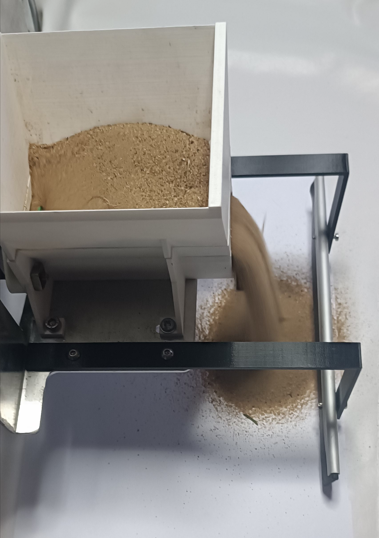
\includegraphics[width=\textwidth]{figures/sand_dispensing.png}
        \caption{Dispenser in operation.}
        \label{fig:dispenser_action}
    \end{subfigure}
    \hfill
    \begin{subfigure}[b]{0.49\textwidth}
        \centering
        \includegraphics[width=\textwidth]{figures/sand_volume.png}
        \caption{Measured volume after a 10-second run.}
        \label{fig:dispensed_volume}
    \end{subfigure}
    \caption{The dispenser flow rate test. The dispenser in operation (a) and the resulting material collected in a measuring cup (b), showing a volume of approximately 200 ml.}
    \label{fig:dispenser_test}
\end{figure}

\textbf{Configuration.}
For this test, the stepper motor was configured using the simplified Arduino firmware, which uses hardcoded parameters for reliability. The motor's maximum speed was set to 2000 steps/second with an acceleration of 2000 steps/second².

\textbf{Results.}
The test was repeated multiple times, and the dispenser demonstrated a high level of consistency. In each 10-second run, it dispensed an average of 200 ml of the sand-seed mixture. This is equivalent to 200 cm³, as 1 milliliter is equal to 1 cubic centimeter. This result establishes a consistent flow rate of approximately 20 cm³/second.

\textbf{Controllability.}
This consistent flow rate proves that the amount of dispensed material can be controlled simply by varying the motor's run time. For example, to dispense the 110 cm³ required to fill the test box from the volume experiment, the motor would need to be run for approximately 5.5 seconds (110 cm³ / 20 cm³/s).

While the full closed-loop system—where the robot measures a divot's volume and automatically calculates the required dispensing time—was not completed, this experiment successfully validates that the mechanical dispenser is both consistent and controllable, making it a viable mechanism for the final system.


\section{Overall Performance of the GolfBot Prototype}
